\chapter{Introducción}\label{ch:Introducción}

\section{Antecedentes}
En las últimas décadas, el avance tecnológico ha permeado de manera significativa en diversos ámbitos de la sociedad, transformando la forma en que interactuamos con el mundo que nos rodea. Uno de los campos donde esta revolución ha sido más evidente es en el ámbito educativo, donde la integración de la tecnología se ha convertido en un tema de relevancia ineludible. Brito \cite{Brito2015} resalta que la emergencia de la cultura digital ha traído consigo profundas transformaciones en la forma en que concebimos la producción, circulación y apropiación del conocimiento, desafiando las estructuras y valores culturales previamente establecidos.

A lo largo del siglo XX, se han iniciado programas para incorporar herramientas tecnológicas en las escuelas de educación básica en México, pero su éxito tanto en términos operativos como pedagógicos ha sido limitado. Esto se atribuye, en parte, a la rigidez de las instituciones escolares, las cuales han enfrentado dificultades para replantear los modelos de socialización que tradicionalmente han prevalecido en el ámbito educativo\cite{Trejo-Quintana2020}.

La llegada de internet, las computadoras y los dispositivos digitales ha abierto un abanico de posibilidades en la educación. La revolución tecnológica de las últimas cuatro décadas ha llevado a la necesidad de integrar dispositivos de comunicación e información en los procesos educativos, considerándose incluso como la única vía para expandir el acceso al conocimiento de manera eficiente y veloz\cite{Trejo-Quintana2020}.

En este entorno, la educación STEM (Ciencia, Tecnología, Ingeniería y Matemáticas), se presenta como un pilar fundamental. Este enfoque interdisciplinario no solo se limita al ámbito académico, sino que también incorpora contextos y situaciones relevantes para la vida cotidiana de los estudiantes, así como los materiales necesarios para su comprensión y aplicación\cite{Sanchez2018}. Desde la perspectiva de Zamorano Escalona, García Cartagena y Reyes González \cite{Zamorano2018}, la educación STEM, o STEAM al incluir las Artes, busca nutrir a la industria científica y tecnológica con recursos humanos creativos. Esto se logra al aumentar el interés de los estudiantes y al desarrollar habilidades esenciales del siglo XXI, fundamentales para estimular el progreso científico-tecnológico, a través de una integración interdisciplinaria de ciencias, tecnología, matemáticas, artes e ingeniería que vincula los contenidos con las experiencias de vida de los estudiantes.

La introducción de la realidad virtual (RV) en este contexto educativo no solo representa un avance tecnológico, sino una oportunidad para superar barreras y maximizar el potencial de la enseñanza. Aunque es cierto que la accesibilidad a esta tecnología puede ser un desafío, su implementación estratégica abre un abanico de posibilidades educativas inexploradas. La RV no solo ofrece experencias inmersivas, sino que también brinda la capacidad de simular situaciones y entornos complejos. Esto la convierte en una herramienta invaluable para la capacitación, investigación y creación de soluciones innovadoras, no solo en el ámbito académico sino también en la industria y el mundo profesional \cite{Zapatero2011}.

\section{Planteamiento del Problema}
Ante la falta de interés y comprensión en la química inorgánica entre los estudiantes, se plantea el desarrollo de un prototipo de simulador de laboratorio en realidad virtual. Esta herramienta busca ofrecer una experiencia educativa más interactiva y atractiva, permitiendo a los estudiantes interactuar con elementos químicos y comprender conceptos tanto básicos como clave en un entorno virtual controlado. El objetivo es revitalizar el interés por esta materia y mejorar el aprendizaje de esta disciplina.

\section{Solución Propuesta}
Un prototipo de simulador de laboratorio de química inorgánica en realidad virtual. Los usuarios podrán realizar experimentos específicos, interactuar con los elementos y observar las reacciones en un entorno controlado.

\begin{itemize}
  \item Prototipo de Simulador en Realidad Virtual de Química Inorgánica que consta de:
    \begin{itemize}
        \item Tabla periódica interactiva.
        \item Interfaz de usuario.
        \item Algoritmos de simulación.
        \item Ejercicios de química inorgánica.
    \end{itemize}
  \item Documentación Técnica.
  \item Manual de Usuario.
  \item Pruebas y validación.
\end{itemize}

\begin{figure}[thbp]
    \centering
    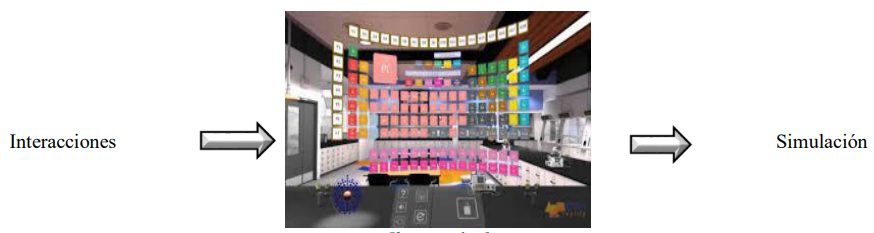
\includegraphics[width=\textwidth]{img/chapter01/Sistema.png}
    \caption{Esquema de Solución.}\label{fig:Esquema}
\end{figure}
\newpage
\section{Objetivos}

\subsection{General}
Desarrollar un prototipo de simulador en realidad virtual que permita a los usuarios interactuar con elementos químicos, combinarlos y observar sus reacciones en un entorno virtual controlado. Este simulador proporcionará una representación visual y práctica de los conceptos clave de la química inorgánica, con el propósito de complementar la comprensión teórica sin sustituir la experimentación en el laboratorio. Limitado a un contexto demostrativo, no esta diseñado para su implementación en entornos educativos formales.


\subsection{Específicos}
\begin{enumerate}[i]
  \item Modelado e integración de una tabla periódica interactiva para una selección dináminca de elementos químicos.
  \item Diseño de la Interfaz de Usuario (IU) para una interacción intuitiva con elementos químicos.
  \item Desarrollo e implementación de algoritmos de simulación para la experimentación virtual y observación de reacciones químicas interactivas.
  \item Crear ejercicios de complejidad progresiva para el aprendizaje de conceptos de química inorgánica.
  \item Pruebas y validación del simulador para una experiencia de usuario satisfactoria.
\end{enumerate}

\section{Justificación}
En el ámbito educativo, se identifica la necesidad apremiante de enriquecer la enseñanza de las ciencias, específicamente la química, entre los jóvenes. A pesar de la disponibilidad de múltiples fuentes de información y recursos audiovisuales para complementar el aprendizaje, persiste la preocupación por la falta de interés de un considerable número de jóvenes en las ciencias. Esta apatía hacia la disciplina puede estar obstaculizando la comprensión profunda y el entusiasmo por aprender sobre la química inorgánica.

En respuesta a este desafío, el proyecto propone una solución innovadora. Mediante una experiencia educativa e interactiva en realidad virtual, se busca abordar la falta de interés al ofrecer una perspectiva diferente y cautivadora de la disiplina. Al proporcionar a los jóvenes una herramienta que les permita interactuar con elementos químicos, combinarlos y observar sus reacciones en un entorno virtual controlado, se fomenta una comprensión más práctica y atractiva de los conceptos.

Esta iniciativa no solo complementa el aprendizaje teórico, sino que también busca revitalizar la motivación intrínseca de los estudiantes hacia las ciencias, en particular la química. Al hacerlo, se aspira a cultivar un ambiente de aprendizaje más estimulante y participativo, que inspire a los estudiantes a explorar y comprender de manera más profunda los principios fundamentales de la química inorgánica.

\newpage
\section{Estado del arte}

\subsection{VRLab Academy}
VRLab Academy se destaca como una empresa líder en innovación tecnológica educativa, especializada en el desarrollo de contenido de experimentos de realidad virtual con propósitos científicos y educativos. Su compromiso se centra en proporcionar a los estudiantes una experiencia de laboratorio virtual auténtica que les permita llevar a cabo experimentos y mejorar sus habilidades en un entorno interactivo, seguro y educativo.

\begin{figure}[thbp]
    \centering
    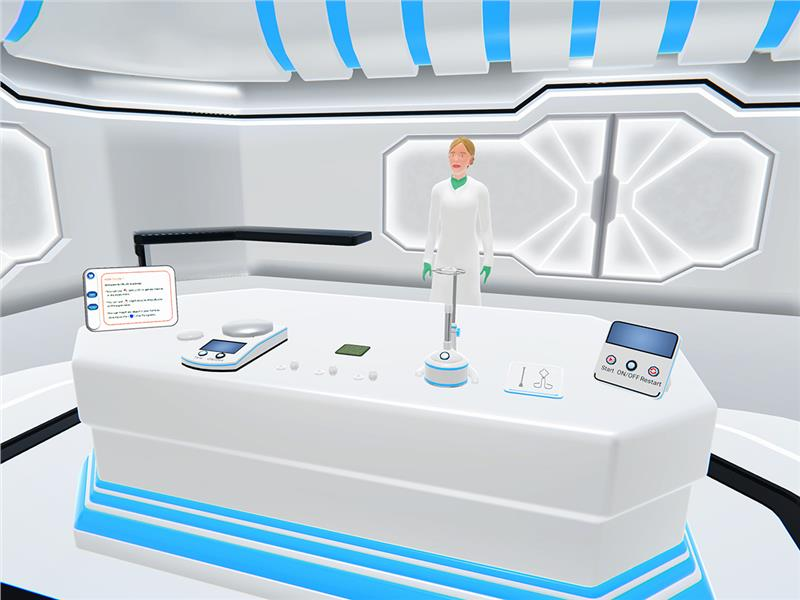
\includegraphics[width=0.8\textwidth, height=8cm]{img/chapter01/Chemistry_Lab_-_VRLab_Academy.jpg}
    \caption{Simulador VRLab Academy.}\label{fig:Esquema}
\end{figure}

El enfoque de VRLab Academy se basa en la utilización de datos en tiempo real, fórmulas científicas verídicas y resultados reales. Los estudiantes tienen la capacidad de guardar y compartir los datos obtenidos durante sus experimentos.

La plataforma de VRLab Academy ofrece dos versiones de sus experimentos: VR y PC. La versión de realidad virtual requiere un dispositivo de realidad virtual como Oculus o HTC, mientras que la versión para PC solo necesita una computadora o portátil con conexión a Internet. Esta variedad de opciones permite adaptarse a las diferentes necesidades y recursos disponibles para los estudiantes.

\newpage
\subsection{Garg Lab VR Chem}

Grag Lab VR Chem es una iniciativa desarrollada por el equipo de químicos orgánicos de la Universidad de California, Los Ángeles (UCLA). Esta plataforma de realidad virtual ha sido creada con el propósito de mejorar el aprendizaje de la química orgánica, ofreciendo a los estudiantes la posibilidad de interactuar con modelos moleculares en un entorno tridimensional.

La aplicación guía a los estudiantes a través de un entorno virtual donde pueden interactuar con modelos moleculares en 3D. Cada molécula viene acompañada de información relevante sobre su función y su presencia en la vida cotidiana, proporcionando contexto adicional para el aprendizaje.

\begin{figure}[thbp]
    \centering
    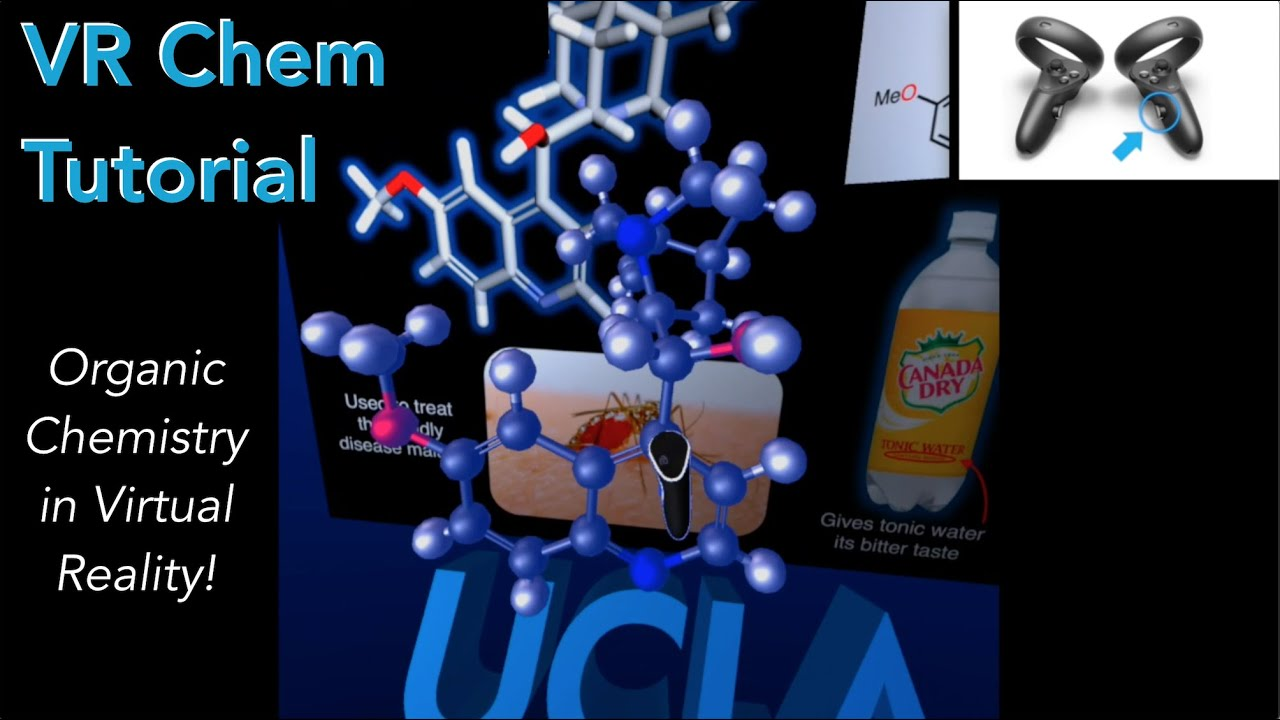
\includegraphics[width=0.8\textwidth, height=8cm]{img/chapter01/Garg_Lab_VR_Chem.jpg}
    \caption{Aplicación VR Chem.}\label{fig:Esquema}
\end{figure}

VR Chem ofrece una ventaja significativa en la comprensión de las estructuras moleculares en 3D, ya que permite a los estudiantes modelar moléculas complejas de una manera interactiva. La aplicación es compatible con una variedad de dispositivos de realidad virtual, incluyendo HTC VIVE, Windows Mixed Reality, Oculus Rift, Oculus Quest, PlayStation VR y Valve Index.

\newpage
\subsection{PraxiLabs}

PraxiLabs es una plataforma educativa que ofrece laboratorios virtuales interactivos en diversas disciplinas científicas, incluyendo química. Esta innovadora plataforma permite a los estudiantes llevar a cabo experimentos virtuales de laboratorio sin la necesidad de contar con equipo físico. De esta manera, PraxiLabs ofrece una experiencia práctica segura y accesible desde cualquier lugar con conexión a Internet.

Se trata de un laboratorio virtual en 3D que ofrece simulaciones de física, química y biología, diseñado para facilitar el proceso de enseñanza de la ciencia tanto para educadores como para estudiantes.

PraxiLabs funciona en computadoras de escritorio y portátiles.

\begin{figure}[thbp]
    \centering
    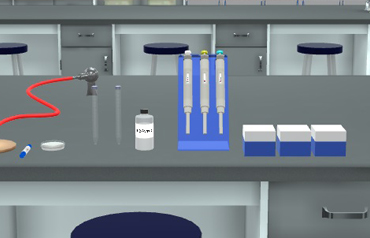
\includegraphics[width=0.8\textwidth, height=8cm]{img/chapter01/Praxi Labs.jpg}
    \caption{Praxi Labs - Laboratorio de Química Inorgánica.}\label{fig:Esquema}
\end{figure}

Se requiere una conexión a Internet confiable para cargar los experimentos. La velocidad de la conexión determina la rapidez de carga. Una vez que el experimento está cargado, no es necesario seguir conectado a Internet, a menos que se utilicen archivos multimedia proporcionados.

\newpage
\subsection{Laboratorio Virtual de Experimentación Química UPM}

El Laboratorio Virtual de Experimentación Química de la UPM es una herramienta educativa que simula un laboratorio real para realizar prácticas de análisis de elementos tóxicos en muestras de suelo. Esta alternativa virtual ofrece mayor seguridad y eficiencia que las prácticas presenciales, ya que reduce riesgos y tiempos de experimentación.

Los estudiantes participan en dos etapas de práctica. En la primera, acceden a material audiovisual y al quimitrivial-UPM desde mesas con ordenadores, además de utilizar un laboratorio equipado con instrumentos básicos de química. Una vez completada esta fase, acceden a los módulos de preparación e instrumentación, donde realizan un procedimiento real para determinar elementos tóxicos en muestras de suelo contaminado. Esto incluye la mineralización de la muestra en un horno de microondas y el análisis por ICP-AES.

\begin{figure}[thbp]
    \centering
    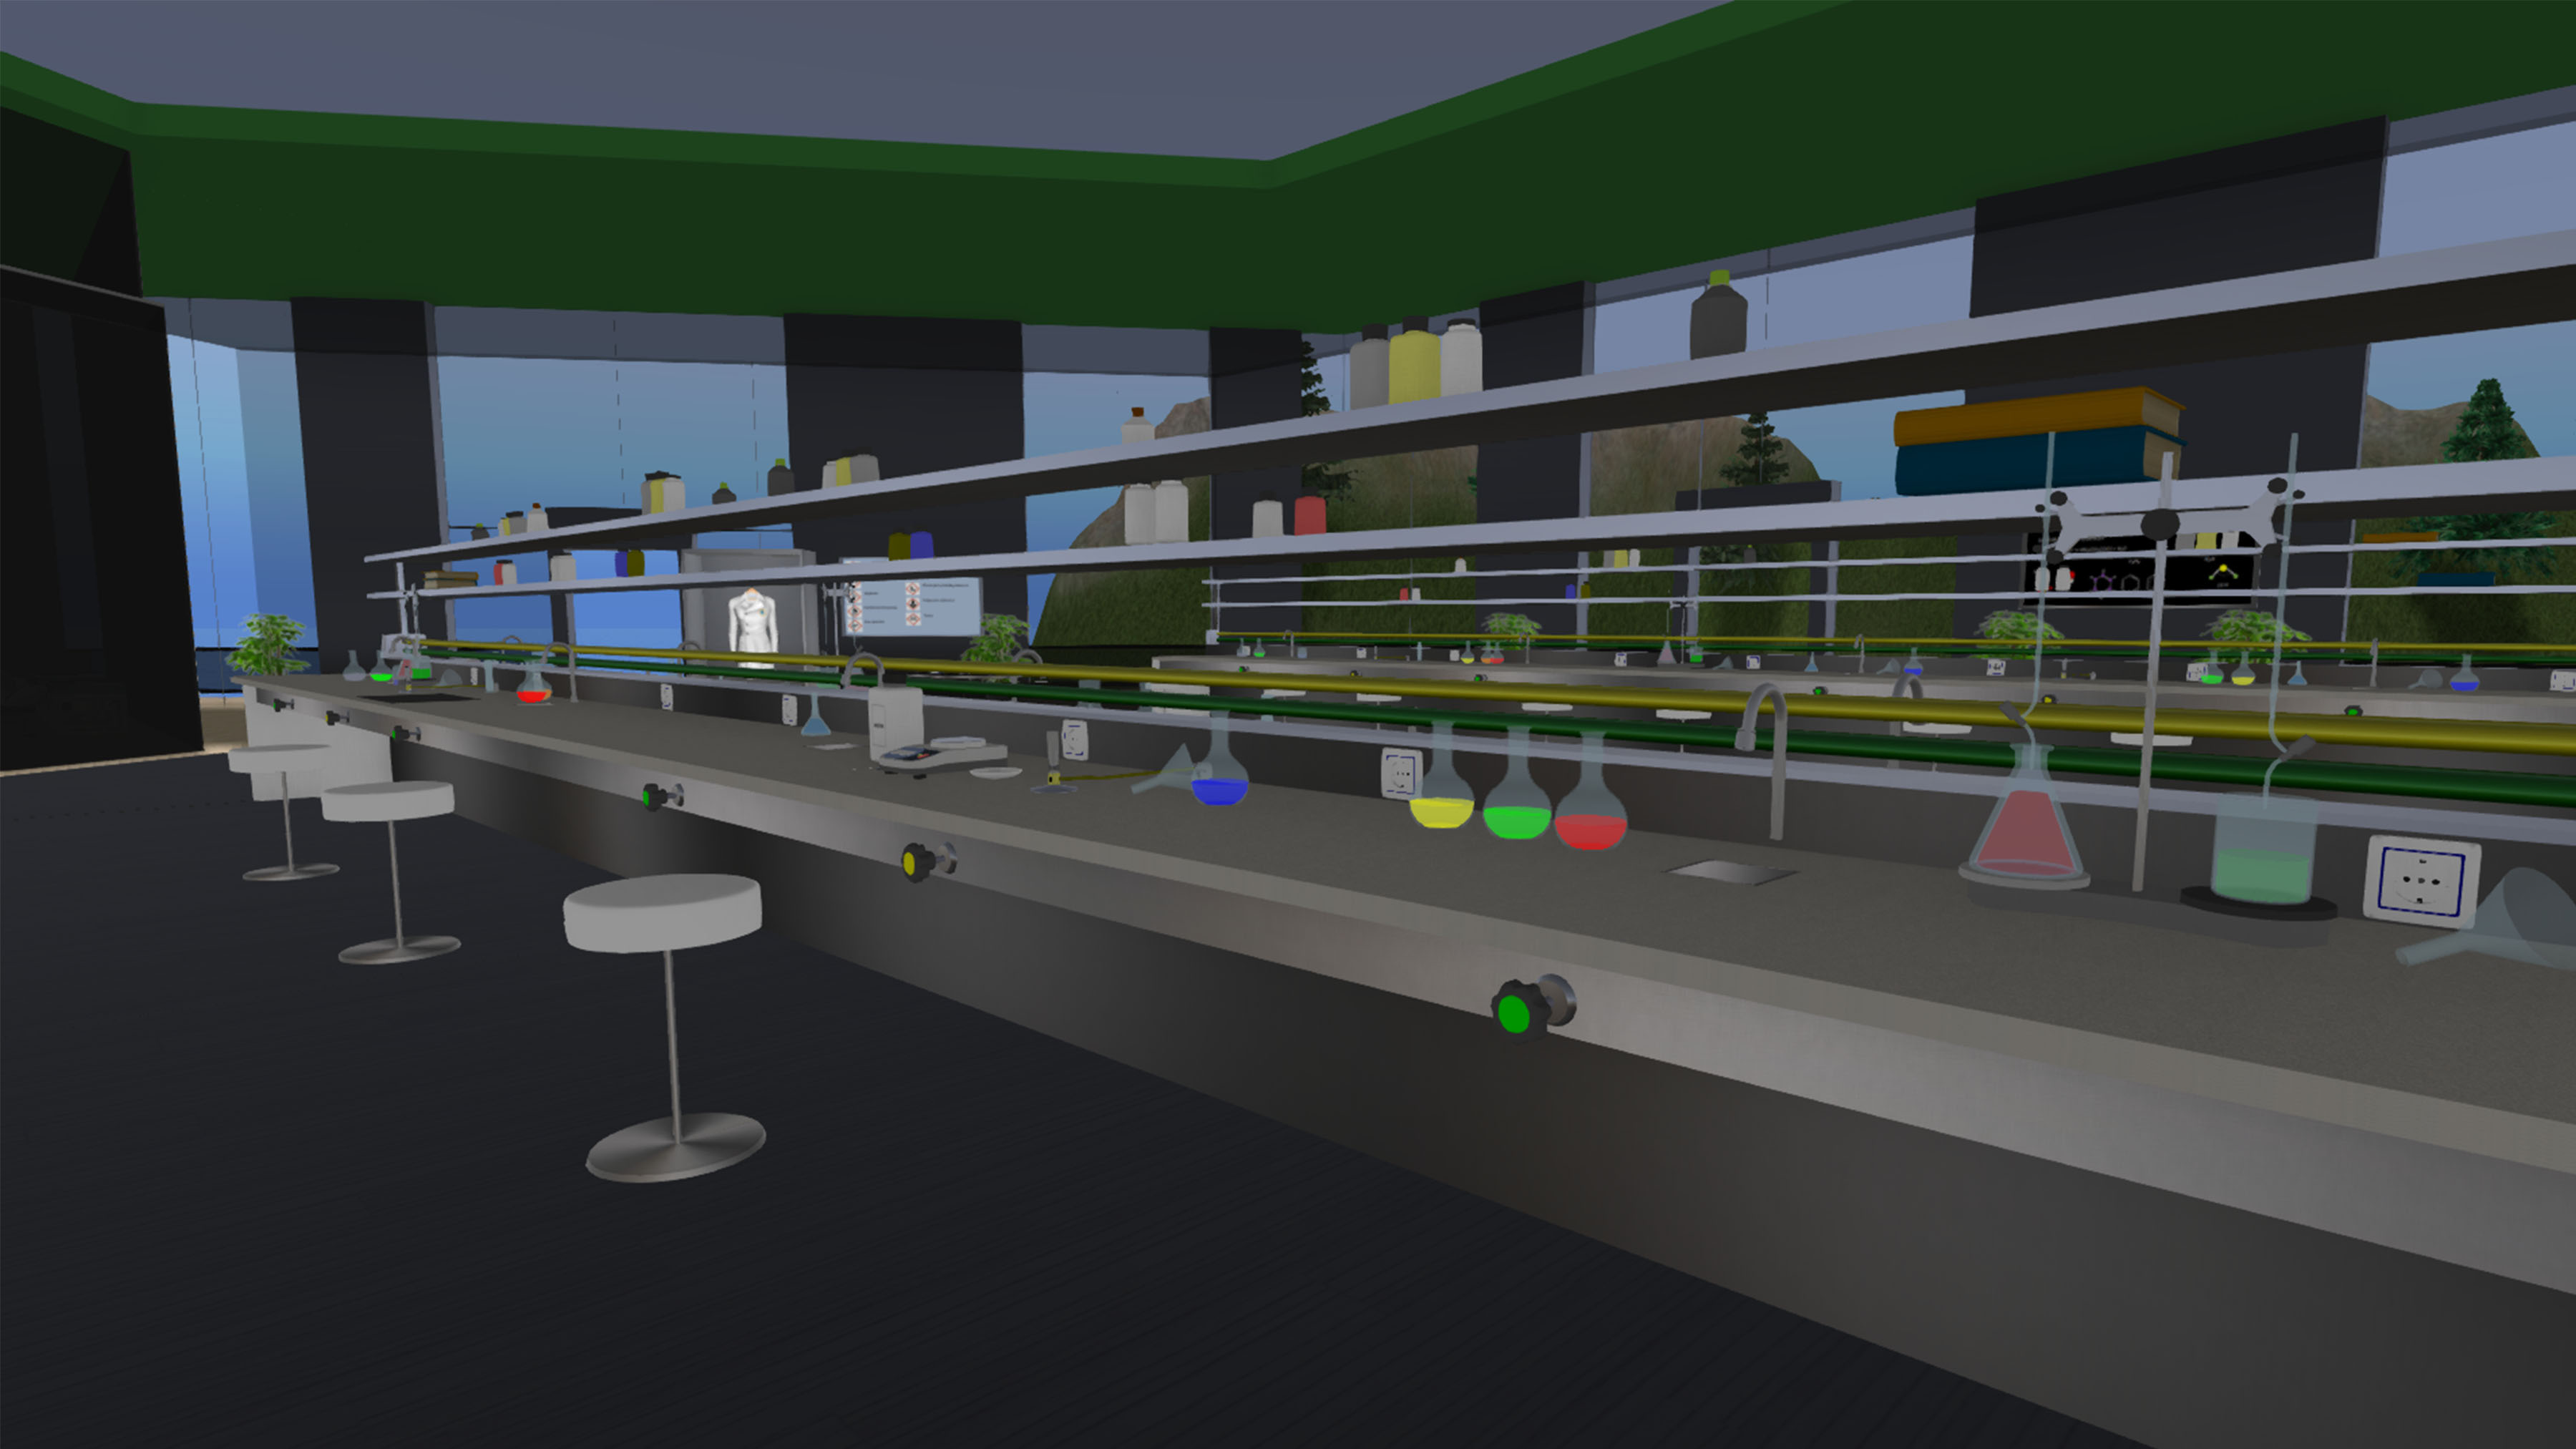
\includegraphics[width=0.8\textwidth, height=8cm]{img/chapter01/UPM.jpg}
    \caption{Experimentación Química UPM.}\label{fig:Esquema}
\end{figure}

Los estudiantes ingresan al laboratorio virtual desde sus ordenadores utilizando sus cuentas institucionales UPM con el Sistema de Inicio de Sesión Único (SSO). La plataforma, construida en Unity 3D y exportada en WebGL, es accesible a través de la mayoría de los navegadores comerciales, sin descargas adicionales. Todo el contenido necesario se descarga automáticamente al conectarse, con una barra de carga indicando el progreso.

\newpage
\subsection{EVA Tech}

Evatech es una plataforma de realidad virtual diseñada para abordar problemas mediante conocimientos científicos. Con un enfoque multidisciplinario, fusiona tecnología, creatividad, pensamiento crítico y habilidades de comunicación.

Esta innovadora herramienta promueve el desarrollo de competencias STEM a través de sesiones de trabajo en equipo en realidad virtual. Dirigida a estudiantes de secundaria y preparatoria, las sesiones interactivas de Evatech refuerzan conceptos científicos y fomentan el aprendizaje práctico y colaborativo.

\begin{figure}[thbp]
    \centering
    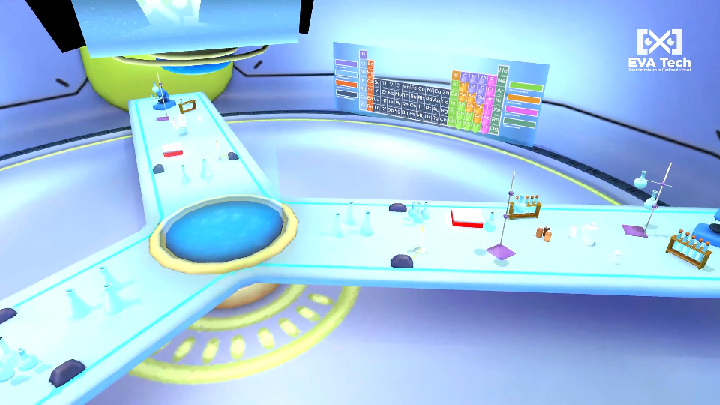
\includegraphics[width=0.8\textwidth, height=8cm]{img/chapter01/Eva_Tech.png}
    \caption{Módulo Química.}\label{fig:Esquema}
\end{figure}

Al utilizar la realidad virtual, Evatech ofrece una experiencia educativa emocionante y efectiva, estimulando nuevas conexiones neuronales al conectar el cuerpo con el razonamiento. Su enfoque en el desarrollo de habilidades motrices y el uso de tecnologías del futuro garantiza un aprendizaje innovador y comprometido con el progreso educativo.

\newpage
\subsection{HoloLab Champions}

HoloLAB Champions es un programa de juegos de realidad virtual que transporta a los jugadores a un laboratorio virtual, donde aprenden habilidades prácticas reales para realizar experimentos. Los jugadores compiten en minilabs organizados por Earl, el presentador holográfico con un sentido del humor ingenioso. Diseñado para estudiantes de 14 a 18 años, este juego de un solo jugador puede ser utilizado en entornos grupales en el aula, donde un estudiante juega mientras otros observan, brindan asistencia y toman notas, con la guía del maestro.

El juego consta de dos episodios de 30 a 40 minutos cada uno, diseñados para enseñar habilidades básicas de laboratorio, procedimientos y protocolos. El primer episodio, Chemiluminescence, enseña a los estudiantes a mezclar ingredientes líquidos y sólidos para crear una solución química brillante. El segundo episodio, Identify Unknowns, desafía a los jugadores a identificar correctamente diversas sustancias con información de referencia limitada.

\begin{figure}[thbp]
    \centering
    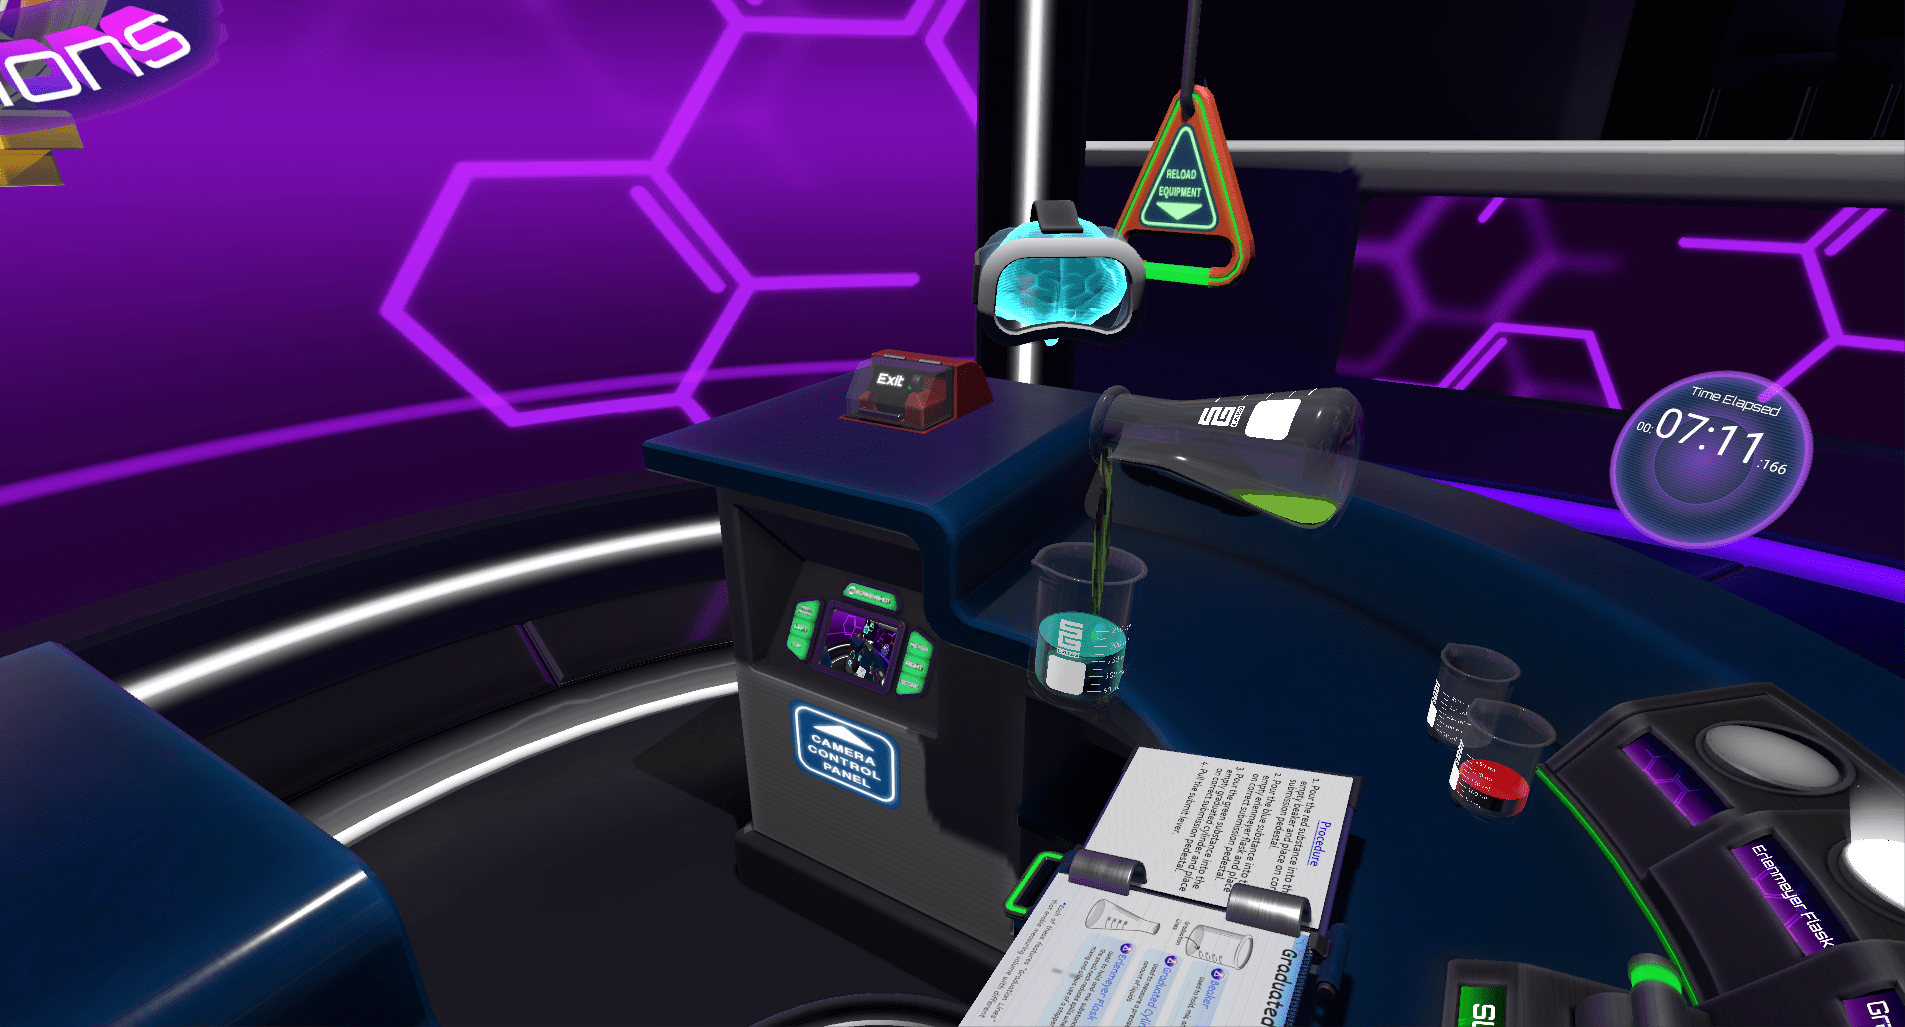
\includegraphics[width=0.8\textwidth, height=8cm]{img/chapter01/hololab-champions_pouring-min.png}
    \caption{HoloLab Champions - Chemiluminescence.}\label{fig:Esquema}
\end{figure}

Financiado parcialmente por una subvención SBIR del Instituto de Ciencias de la Educación del Departamento de Educación de los Estados Unidos, HoloLAB Champions fue desarrollado en asociación con estudiantes, educadores y la RAND Corporation, siguiendo un proceso iterativo para garantizar su efectividad y utilidad educativa.

\newpage
\subsection{Tabla Comparativa}

\begin{table}[H]
  \centering
  \begin{tabular}{|>{\centering\arraybackslash}m{.2\textwidth}|>{\centering\arraybackslash}m{.1\textwidth}|>{\centering\arraybackslash}m{.1\textwidth}|>{\centering\arraybackslash}m{.15\textwidth}|>{\centering\arraybackslash}m{.15\textwidth}|>{\centering\arraybackslash}m{.15\textwidth}|}
    \hline
    \rowcolor{blue_escom}
    Simulador &  Realidad Virtual (VR) &  Hand Tracking &  Etapas Integradas & Idioma & Público Objetivo
 \\
    
    \hline
    \cellcolor{column_color}VRLab Academy & ✓ & ✗ & Visualización, Experimentación & Varios & Estudiantes de Preparatoria y Universidad \\
    
    \hline
    \cellcolor{column_color}Garg Lab VR Chem & ✓ & ✗ & Visualización & Inglés & Estudiantes de pregrado\\
    
    \hline
    \cellcolor{column_color}PraxiLabs & ✗ & ✗ & Experimentación & Inglés y Árabe & Estudiantes de ciencias\\
    
    \hline
    \cellcolor{column_color}Laboratorio Virtual de Experimentación Química UPM & ✗ & ✗ & Balanceo de ecuaciones, Experimentación & Español & Estudiantes universitarios\\
    
    \hline
   \cellcolor{column_color} EVA Tech & ✓ & ✗ & Visualización & Español & Estudiantes de Nivel Básico\\
   
    \hline
    \cellcolor{column_color}HoloLab Champions & ✓ & ✗ & Experimentación & Inglés & Adolescentes y Adultos\\
    
    \hline
    \cellcolor{column_color}TT-2024-B059 & ✓ & ✓ & Visualización, Balanceo de ecuaciones, Creación de compuestos, Experimentación & Español & Adolescentes\\
    \hline
  \end{tabular}
  \caption{Comparativa de simuladores de laboratorios virtuales}
  \label{tab:comparativa}
\end{table}
